\documentclass[10pt,twocolumn]{article}
\usepackage{xeCJK}
\setCJKmainfont[Path=C:/Windows/Fonts/,BoldFont=simhei.ttf,ItalicFont=simkai.ttf]{simsun.ttc}
\setCJKsansfont[Path=C:/Windows/Fonts/]{msyh.ttc}
\setCJKmonofont[Path=C:/Windows/Fonts/]{simfang.ttf}
\usepackage[margin=0.72in,columnsep=0.26in]{geometry}
\usepackage{amsmath,amssymb}
\usepackage{graphicx}
\usepackage{xcolor}
\usepackage{array}
\usepackage[hidelinks]{hyperref}

\definecolor{accent}{RGB}{30,58,138}
\renewcommand{\arraystretch}{1.16}
\renewcommand{\abstractname}{摘要}
\renewcommand{\figurename}{图}
\renewcommand{\tablename}{表}
\renewcommand{\refname}{参考文献}

\title{\Large\bfseries 单机征服《真侍魂》：面向经典格斗街机的硬件感知\\
混合专家架构与物理不变量三局两胜仲裁机制}

\author{侍魂2 AI 项目组（\texttt{footballqq}）\\
\small 开源发布仓库：\url{https://github.com/footballqq/samsho2-moe-ai}}
\date{2026年11月}

\begin{document}
\maketitle

\begin{abstract}
在单机算力受限的条件下，为经典街机格斗游戏构建自主智能体面临多重叠加挑战：极高的单刀伤害致命性、跨角色梯度冲突、动态镜头缩放引发的画面血条失真，以及连续三局两胜（Best-of-3, Bo3）赛制中隐蔽的评测仲裁漏洞。本文作为一篇系统工程与实证方法论研究论文，完整记录了基于 MAME 0.281 模拟器构建 SNK Neo-Geo 经典武器格斗游戏《真侍魂：霸王丸地狱变》（\texttt{samsho2}）自主 AI 系统的全过程。针对单机从零训练单体 PPO（Proximal Policy Optimization）在实践中普遍陷入“角落消极避战”与“跨对手灾难性遗忘”的困境，本文提出了一套四层解耦系统架构：（1）基于 Neo-Geo WRAM 物理内存直读的硬件级实体感知（\texttt{UID+0xBB} 权威逻辑血量、归一化水平距离、命中伤害锁存器，以及实机标定的 \texttt{0x00}--\texttt{0x10} 硬件角色 ID 映射）；（2）9 维半马尔可夫决策过程（SMDP）语义战斗意图空间；（3）物理级隔离的混合专家（MoE）路由器，结合分回合策略与基于实时距离的闭环反应控制器（\texttt{DistanceReactivePolicy}）；（4）针对两起真实评测事故（BUG-17 超时判定反转与 BUG-18 转场闪烁幻影回合）形式化设计的物理不变量 Bo3 状态机（\texttt{Bo3MatchController}）。在 1$\times$ 原速 60~FPS 实机 MAME 仿真中，AI 霸王丸实现了全员 16/16 对手真 Bo3 100\% 击破（全部通过 18.0 秒战后结算录像与中英双语时间轴校验），并实现了零抢键冲突的真双人 2P VS 人机实机对抗。最后，本文诚实剖析了开环序列专家面对人类动态变招的泛化短板，并给出了以现有 MoE 资产反哺 PPO 与离线强化学习的演进路线。
\end{abstract}

\noindent\textbf{关键词}---格斗游戏 AI；混合专家模型（MoE）；半马尔可夫决策过程（SMDP）；街机仿真；评测可信性；强化学习

\section{引言}
经典 2D 街机格斗游戏因其严苛的 60~Hz 帧级反应窗口、非对称角色机制与非传递性（剪刀石头布式）博弈结构，长期以来一直是序贯决策与强化学习的重要测试基准~\cite{lu2013fightingice,vinyals2019alphastar}。在众多经典作品中，SNK 于 1994 年推出的 Neo-Geo 武器格斗代表作《真侍魂》（\texttt{samsho2}）具备尤为严酷的力学特征：单记重斩即可削去角色 30\%--50\% 血量；双方拉距时镜头自动缩放导致像素血条形变；而在三局两胜（Bo3）赛制中，游戏采用\emph{非对称局间回血}机制——败者血条回满，胜者仅保留残血进入下一局。

在项目早期的单机 PPO~\cite{schulman2017ppo} 从零训练实验中，我们反复遭遇三大工程阻碍：（1）\emph{消极避战局部极小}——挥空、重复与受伤惩罚叠加后，缩在版边死防的期望回报高于主动出刀；（2）\emph{跨角色梯度冲突}——16 名对手截然相反的克制打法在共享权重中剧烈互相擦除；（3）\emph{单机仿真吞吐瓶颈}。更值得警惕的是，研发期间发生的两起隐蔽评测故障（BUG-17 超时符号反转与 BUG-18 转场闪烁幻影回合）揭示了“未经物理不变量守卫的自动化指标极易制造虚假高胜率”。

作为一篇立足单机工程实践的系统与实证方法论论文，本文的核心贡献如下：
\begin{enumerate}
    \item \textbf{硬件级 WRAM 实体感知与 SMDP 语义抽象}：通过 MAME 0.281 Lua TCP 锁步网桥直读 Neo-Geo WRAM 权威内存，并将逐帧按键压缩为 9 维语义战斗意图。
    \item \textbf{物理隔离 MoE 与闭环距离反应专家}：将 16 名对手解耦为独立 JSON 策略配置，并提出闭环 \texttt{DistanceReactivePolicy} 攻克全屏站位 Boss（罗将神水姬与席格）。
    \item \textbf{物理不变量 Bo3 仲裁机制}：从真实故障中提炼出六大评测铁律与三层守卫状态机，彻底消除超时误判与幻影第 2 局。
    \item \textbf{16/16 全员实机验证、真 2P VS 对战与开源发布}：通过 60~FPS 完整 Bo3 录像（含 18.0~s 结算画面与双语字幕）完成全员验证，落地零抢键 2P VS 人机对抗，并开源完整纯净代码库。
\end{enumerate}

\section{相关工作}
\textbf{格斗游戏 AI 与街机仿真测试床。} 格斗 AI 研究涵盖 FightingICE~\cite{lu2013fightingice} 平台上的规则与蒙特卡洛树搜索、基于 Gym-Retro / MAME 桥接的《街头霸王》深度强化学习，以及超大规模自对弈联赛~\cite{vinyals2019alphastar}。与暴露干净 API 的研究模拟器不同，在 MAME 中运行真实 Neo-Geo 街机 ROM 需要对底层 WRAM 内存进行逆向标定，并妥善处理非确定性的街机过场与局间动画。

\textbf{SMDP 宏动作与混合专家模型。} 基于选项框架与半马尔可夫决策过程（SMDP）~\cite{sutton1999options} 的时间抽象能显著缩短高频控制的有效决策步长。混合专家架构（MoE）~\cite{jacobs1991moe} 通过将异质任务路由至独立子模块来抑制负迁移。在本系统中，基于 WRAM 对手 ID 的静态路由实现了 16 位角色间的物理零干扰。

\textbf{评测可信性与离线强化学习。} 奖励作弊与评测器漏洞是强化学习中的已知系统性风险~\cite{amodei2016concrete}。本文对 BUG-17 与 BUG-18 的工程复盘呼应了引入独立物理不变量与人工目视复核的必要性。面向后续泛化演进，行为克隆、Kickstarting 策略蒸馏~\cite{schmitt2018kickstarting}、Go-Explore 残局回溯~\cite{ecoffet2021goexplore} 及隐式 Q 学习（IQL）~\cite{kostrikov2022iql} 为 MoE 资产反哺神经网络 RL 提供了清晰路径。

\begin{figure*}[t]
    \centering
    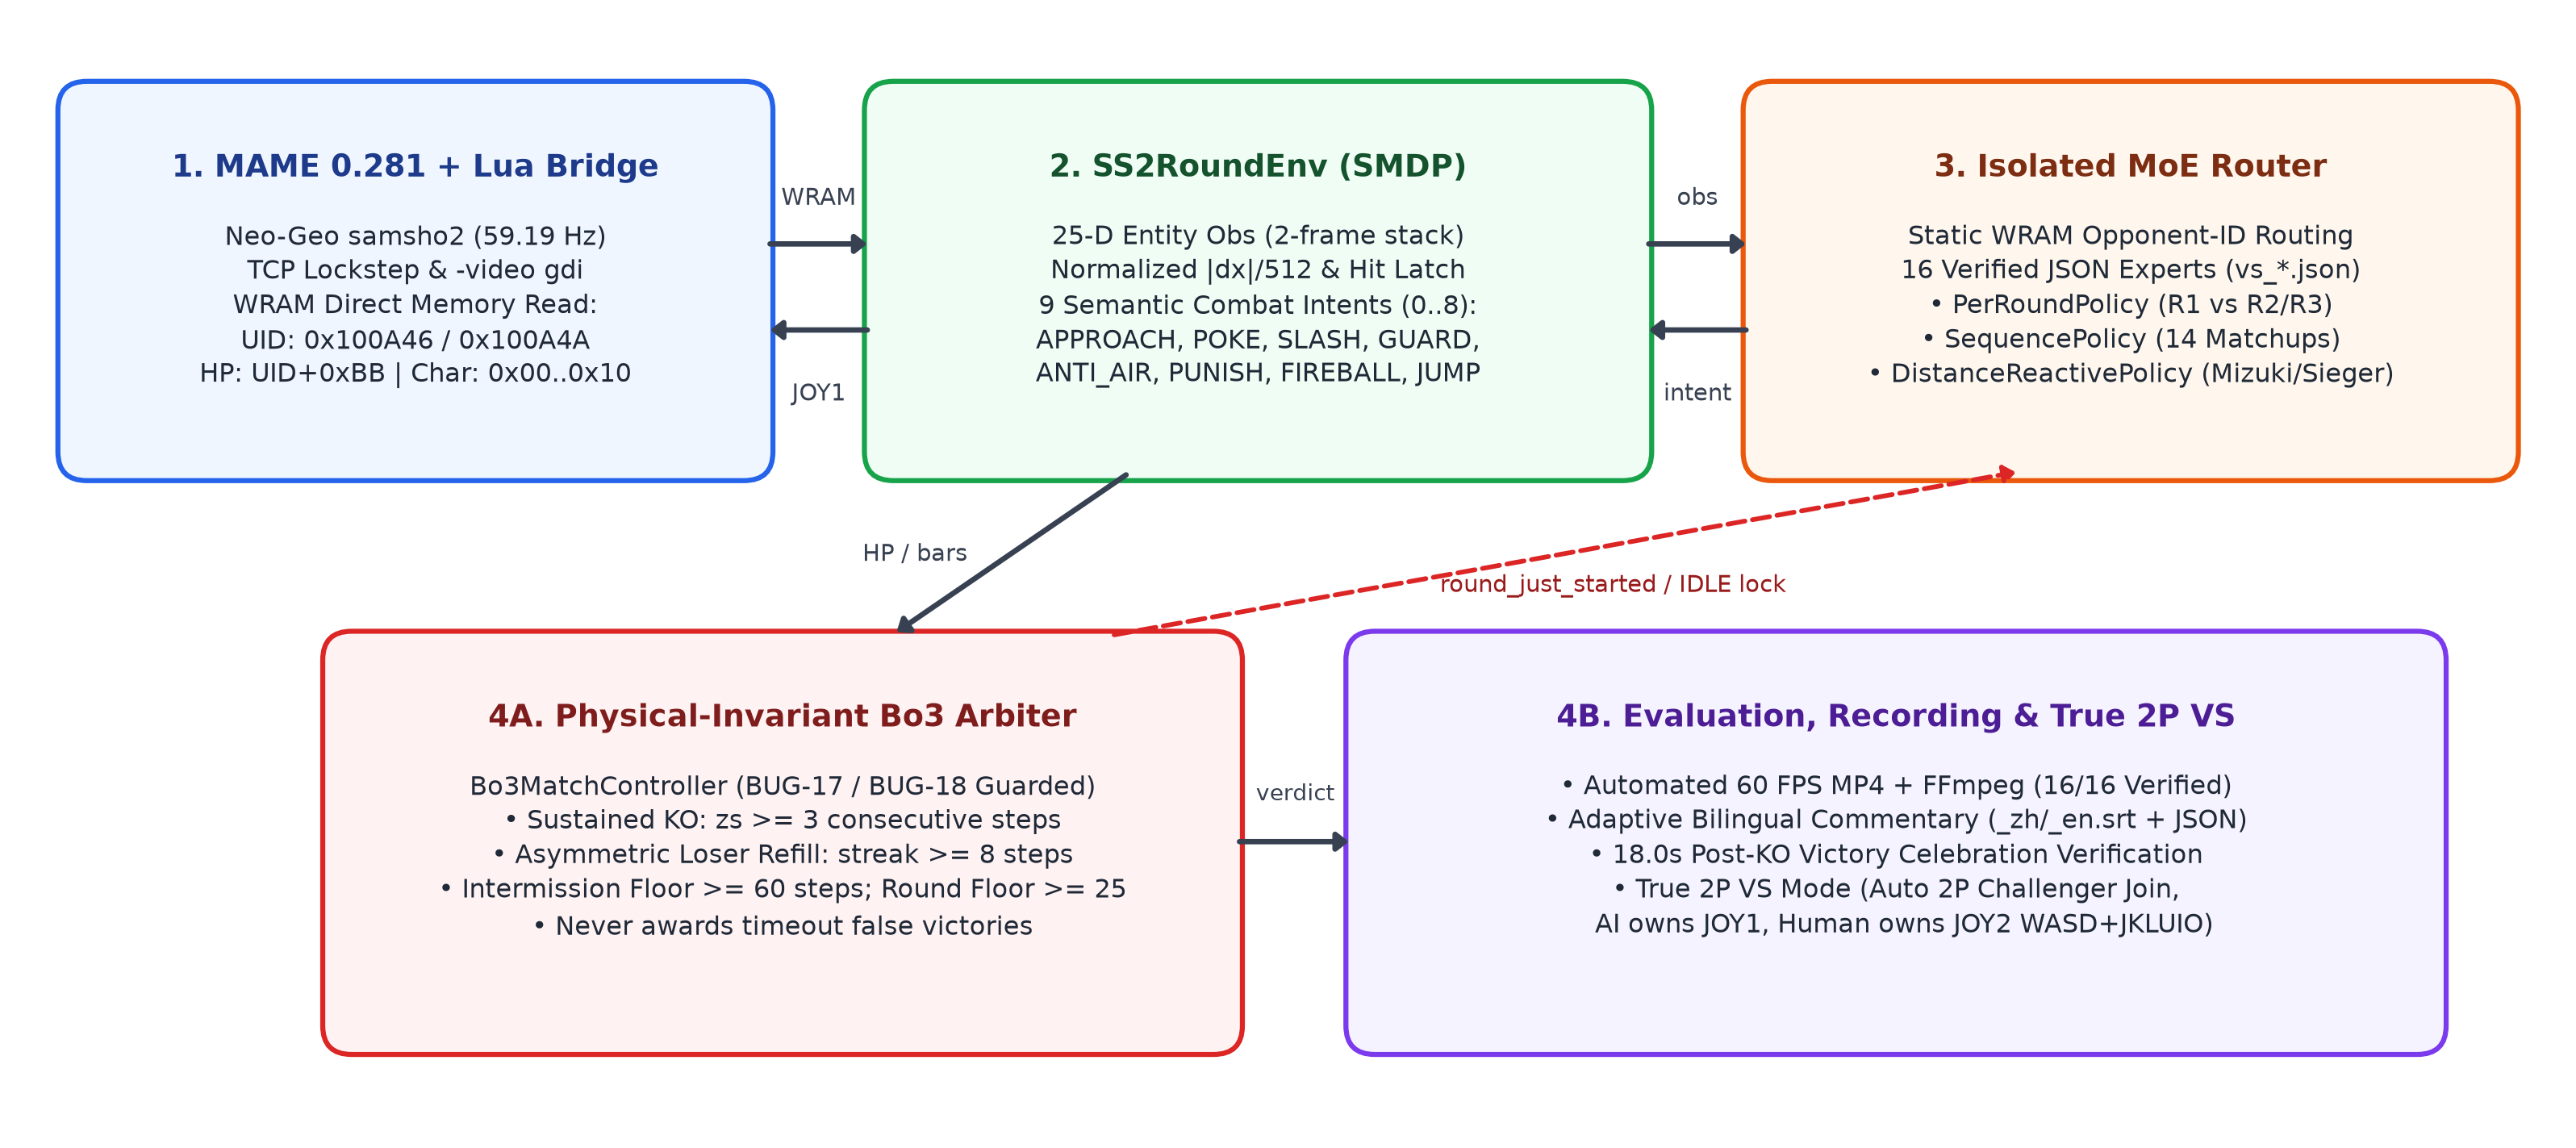
\includegraphics[width=0.96\textwidth]{figures/fig1_architecture.png}
    \caption{《真侍魂》MoE 智能体四层系统架构：（1）MAME 0.281 Lua TCP 锁步网桥与 WRAM 直读；（2）\texttt{SS2RoundEnv} SMDP 环境（25 维实体观测与 9 维战斗意图）；（3）物理隔离 MoE 路由器（结合分回合序列与闭环距离反应策略）；（4）物理不变量 Bo3 仲裁器，驱动 60~FPS 多模态录播与真 2P VS 人机对战。}
    \label{fig:arch}
\end{figure*}

\section{系统架构与硬件级内存感知}
图~\ref{fig:arch} 展示了系统的整体四层架构。

\subsection{MAME 0.281 锁步网桥与后台稳定性}
底层 Lua 网桥（\texttt{mame/bridge.lua}）通过本地动态端口 TCP Socket 与 Python 锁步通信。为确保 Windows 后台无人值守批量录制稳定运行，系统强制采用纯软件 GDI 渲染（\texttt{-video gdi}）替代 Direct3D，彻底规避锁屏或显示器休眠导致的显卡驱动 TDR 挂起崩溃；同时借助 Win32 Job Object（\texttt{win32\_process.py}）保证进程退出时自动回收全部子进程，杜绝孤儿进程残留。

\subsection{Neo-Geo WRAM 权威实体直读}
基于视觉像素的血条解析在《真侍魂》中存在镜头缩放形变、怒气闪烁变色以及 15--30 帧渐变动画延迟三大硬伤。本系统直接读取 Neo-Geo WRAM 中的物理实体字段：
\begin{itemize}
    \item \textbf{动态实体指针}：1P 与 2P 实体基址（\texttt{UID}）分别位于 \texttt{0x100A46} 与 \texttt{0x100A4A}。
    \item \textbf{权威逻辑血量}：\texttt{UID + 0xBB} 为 1 字节无符号整数（标准满血 128，橘右京 164，席格 186）。
    \item \textbf{命中伤害锁存器}：\texttt{0x105ED3} 在攻击命中的当帧立即置位，消除挥空误判。
    \item \textbf{实机标定硬件角色 ID（\texttt{UID + E\_CHAR}）}：对全部 16 个角色存档进行实机探测发现，\texttt{0x0A} 为裁判黑子/保留槽位，导致夏洛特至罗将神水姬的真实硬件 ID 顺延至 \texttt{0x0B}--\texttt{0x10}（\texttt{0x0B}：夏洛特，\texttt{0x0C}：牙神，\texttt{0x0D}：查姆查姆，\texttt{0x0E}：席格，\texttt{0x0F}：和仲，\texttt{0x10}：水姬）。修正该映射表彻底消除了真 2P VS 对战中的识人错位问题。
\end{itemize}

每步环境构造 25 维实体特征并堆叠最近 2 步（共 50 维），包含有符号水平偏移、归一化距离 $|dx|/512$（通道~1）、双方血量比、怒气值、晕眩槽及 6 位角色动作状态标志。

\subsection{9 维 SMDP 语义战斗意图空间}
策略不再输出 60~Hz 原始摇杆位掩码，而是从 9 个符合格斗直觉的语义战斗意图中决策（表~\ref{tab:intents}），由底层招式宏反射层（\texttt{data/mame/movesets/haohmaru.yaml}）在每步 2--8 帧内展开执行。

\begin{table}[t]
\centering
\caption{9 维 SMDP 语义战斗意图空间定义}
\label{tab:intents}
\small
\begin{tabular}{c l l}
\hline
\textbf{编号} & \textbf{意图标识} & \textbf{战术语义与执行功能} \\
\hline
0 & \texttt{APPROACH} & 前冲/前走逼近，压缩立回距离 \\
1 & \texttt{RETREAT}  & 后撤拉开，脱离版边压制 \\
2 & \texttt{POKE}     & 高速轻刺试探，打断对手起手 \\
3 & \texttt{SLASH}    & 核心高伤重斩大劈（A+B） \\
4 & \texttt{ANTI\_AIR} & 升龙弧月斩，精准拦截跳入 \\
5 & \texttt{PUNISH}   & 捕捉对手招式硬直实施确反重击 \\
6 & \texttt{FIREBALL} & 旋风裂斩飞行道具中远程牵制 \\
7 & \texttt{GUARD}    & 站立/下蹲稳固防御架势 \\
8 & \texttt{JUMP}     & 方向性起跳下砸，破除低位牵制 \\
\hline
\end{tabular}
\end{table}

\section{物理隔离 MoE 策略架构}
\subsection{单机单体 PPO 停滞的机理剖析}
当使用单一共享参数 PPO 网络 $\pi_\theta(a|s)$ 混训全部 16 名对手时，两项机制共同导致了训练失败。首先，受伤、挥空与重复惩罚叠加后诱导策略落入局部极小：$\mathbb{E}[R(\text{后退/死防})] > \mathbb{E}[R(\text{主动进攻})]$。其次，不同对手的克制梯度方向彼此尖锐对立：
\begin{equation}
\langle \nabla_\theta J_{\text{地震}},\, \nabla_\theta J_{\text{牙神}} \rangle < 0,
\end{equation}
例如克制地震铁链的主动跳斩压制，面对牙神幻十郎的无敌对空升龙时会立刻遭到毁灭性反杀。

\subsection{分回合序列与闭环距离反应专家}
我们将 16 位对手解耦为独立的 JSON 配置文件（\texttt{models/experts/vs\_<opponent>.json}），由 \texttt{MoEAgent.set\_opponent()} 按对手 ID 静态路由，保证单角色优化对其他 15 位对手绝对零回归。每个专家采用 \texttt{PerRoundPolicy}，监听 \texttt{Bo3MatchController.round\_just\_started} 信号实现回合级指针重置，从而解耦第 1 局先手抢攻与第 2/3 局局间横幅重置后的防反节奏。

对于 14 名对手，分回合前缀+循环序列已足以稳定赢下完整 Bo3。然而在对抗终极 Boss \textit{罗将神水姬}与重甲摔投角色\textit{席格}时，第 2/3 局重置后双方站位拉远至全屏（$|dx| > 250$~px），开环序列会在远处反复挥空。为此，我们在 \texttt{src/mame\_moe.py} 中设计了闭环控制器 \texttt{DistanceReactivePolicy}，实时读取观测中的归一化距离 $d_t = |dx_t|/512$ 动态切换远程逼近与近身斩杀循环：
\begin{equation}
a_t = \begin{cases}
\text{prefix}[t], & t < |\text{prefix}|, \\
\text{far\_loop}[i_f \bmod L_f], & d_t > \tau_{\text{far}}, \\
\text{close\_loop}[i_c \bmod L_c], & d_t \le \tau_{\text{far}}.
\end{cases}
\end{equation}
设定 $\tau_{\text{far}} = 0.22$（\texttt{far\_loop=[0,8,7]}，\texttt{close\_loop=[8,4,3,5]}）后，霸王丸仅用 603 步（78.7~s）便以 2--0 横扫终极 Boss 水姬；设定 $\tau_{\text{far}} = 0.24$（\texttt{far\_loop=[0,3,7]}，\texttt{close\_loop=[4,3,7]}）后，在 969 步（123.7~s）以 2--1 击败席格。

\section{物理不变量三局两胜仲裁机制}
\subsection{真实故障复盘：BUG-17 与 BUG-18}
两起实战评测事故深刻塑造了本系统的仲裁设计：
\begin{itemize}
    \item \textbf{BUG-17（超时判定符号反转）}：早期计时器耗尽判定中大小于号写反，把“残血超时判负”错计为胜利。由于训练奖励、中途评估与终审复用了同一份裁判代码，三级指标互相“自洽印证”出 85\% 的虚假胜率，直到人工观战才暴露实机 0--2 惨败。
    \item \textbf{BUG-18（转场闪烁幻影回合）}：在连续 Bo3 录屏及后续 2P VS 真人测试中，KO 慢动作与切场横幅期间短暂的像素条/内存闪烁会误触发“新一局已开打”，紧随其后的黑屏 3 帧立即被再次判死，导致仅打完 1 局就被误判为 0--2 提前结束。
\end{itemize}

\subsection{六大评测铁律与三层物理守卫}
针对上述教训，我们在工程规范中确立了六大铁律：（1）裁判必须对照游戏本尊可见横幅交叉核对；（2）物理不变量（回合时长下限、血量守恒）必须入单测；（3）胜负测试期望值来自实录而非代码臆推；（4）指标单调向好触发成分审计；（5）人工目视观战为硬发布关卡；（6）单一裁判异常则全链路下线重测。

据此，\texttt{Bo3MatchController}（\texttt{src/bo3\_controller.py}）实现了三层物理不变量守卫：
\begin{enumerate}
    \item \textbf{持续零血与单局下限门禁}：须连续 $z_s \ge 3$ 步血量为 0 方可判 KO，且新局前 25 步（约 0.8~s）内禁止判死，彻底屏蔽切场黑屏。
    \item \textbf{局间最小时长保护}：局间等待强制至少 60 步（约 2.0~s）并锁定 AI 输出 \texttt{IDLE}，跨越 KO 慢动作与胜负横幅期。
    \item \textbf{非对称持续回血校验}：必须检测到上一局\emph{败者}血量回满（$>50\%$ 像素条或 $>60$ WRAM 血量）并连续稳定 8 步（\texttt{\_refill\_streak >= 8}），方可开启下一局。
\end{enumerate}

\begin{figure*}[t]
    \centering
    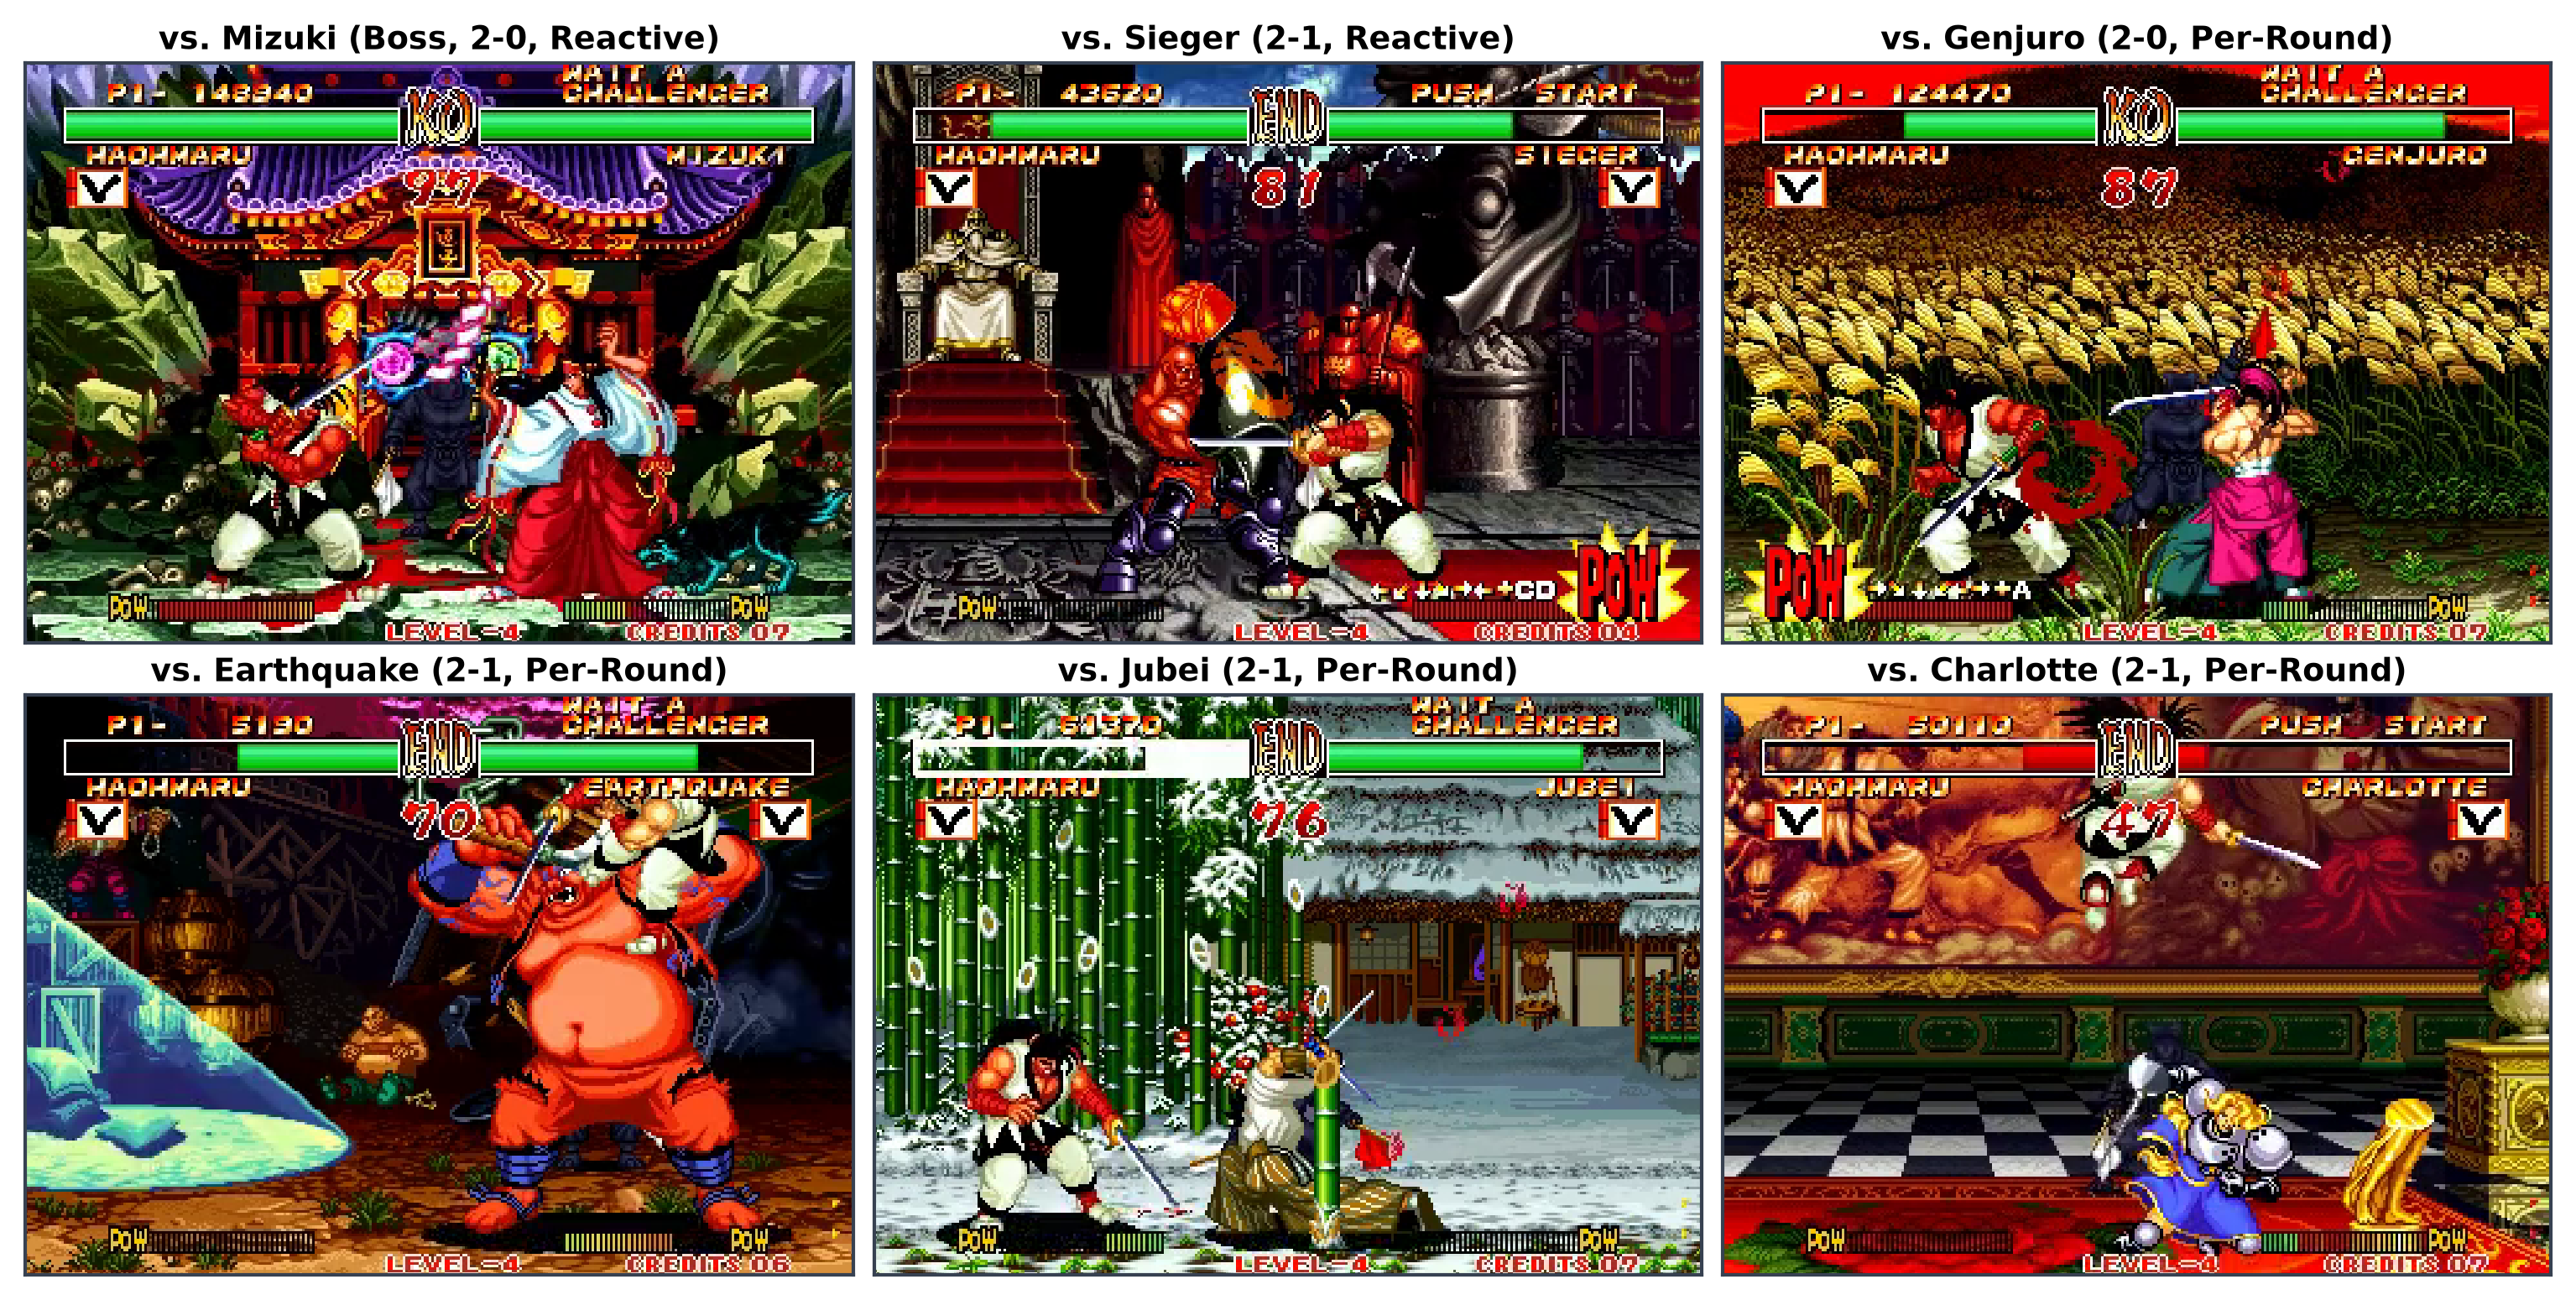
\includegraphics[width=0.96\textwidth]{figures/fig2_gameplay_montage.png}
    \caption{从 16 部 60~FPS 实机验收 Bo3 录像中直接抽取的 6 场代表性实战画面，包含闭环距离反应策略击败终极 Boss 罗将神水姬（2--0）与席格（2--1），以及分回合专家击败牙神幻十郎、地震、柳生十兵卫与夏洛特的实机瞬间。}
    \label{fig:montage}
\end{figure*}

\section{实验评测与实机结果}
\subsection{全员 16/16 实机 Bo3 验收}
所有 16 位对手均通过 \texttt{tools/record\_match\_mp4.py} 在 MAME 0.281 原生 1$\times$ 速率下完成实机 Bo3 录制与验证，并经由 \texttt{ffprobe} 与 \texttt{\_commentary.json} 逐一通过物理门禁核验：比分严格为 \texttt{2-0} 或 \texttt{2-1}，完整时长 $\ge 78$~s，战后强制录制 18.0 秒收刀与大比分结算画面，并同步生成中英双语 SRT 字幕。图~\ref{fig:montage} 展示了 6 场实机画面，图~\ref{fig:perf} 汇总了全员时长与策略分布，表~\ref{tab:results} 列出了全部 16 场实测数据。

\begin{figure}[t]
    \centering
    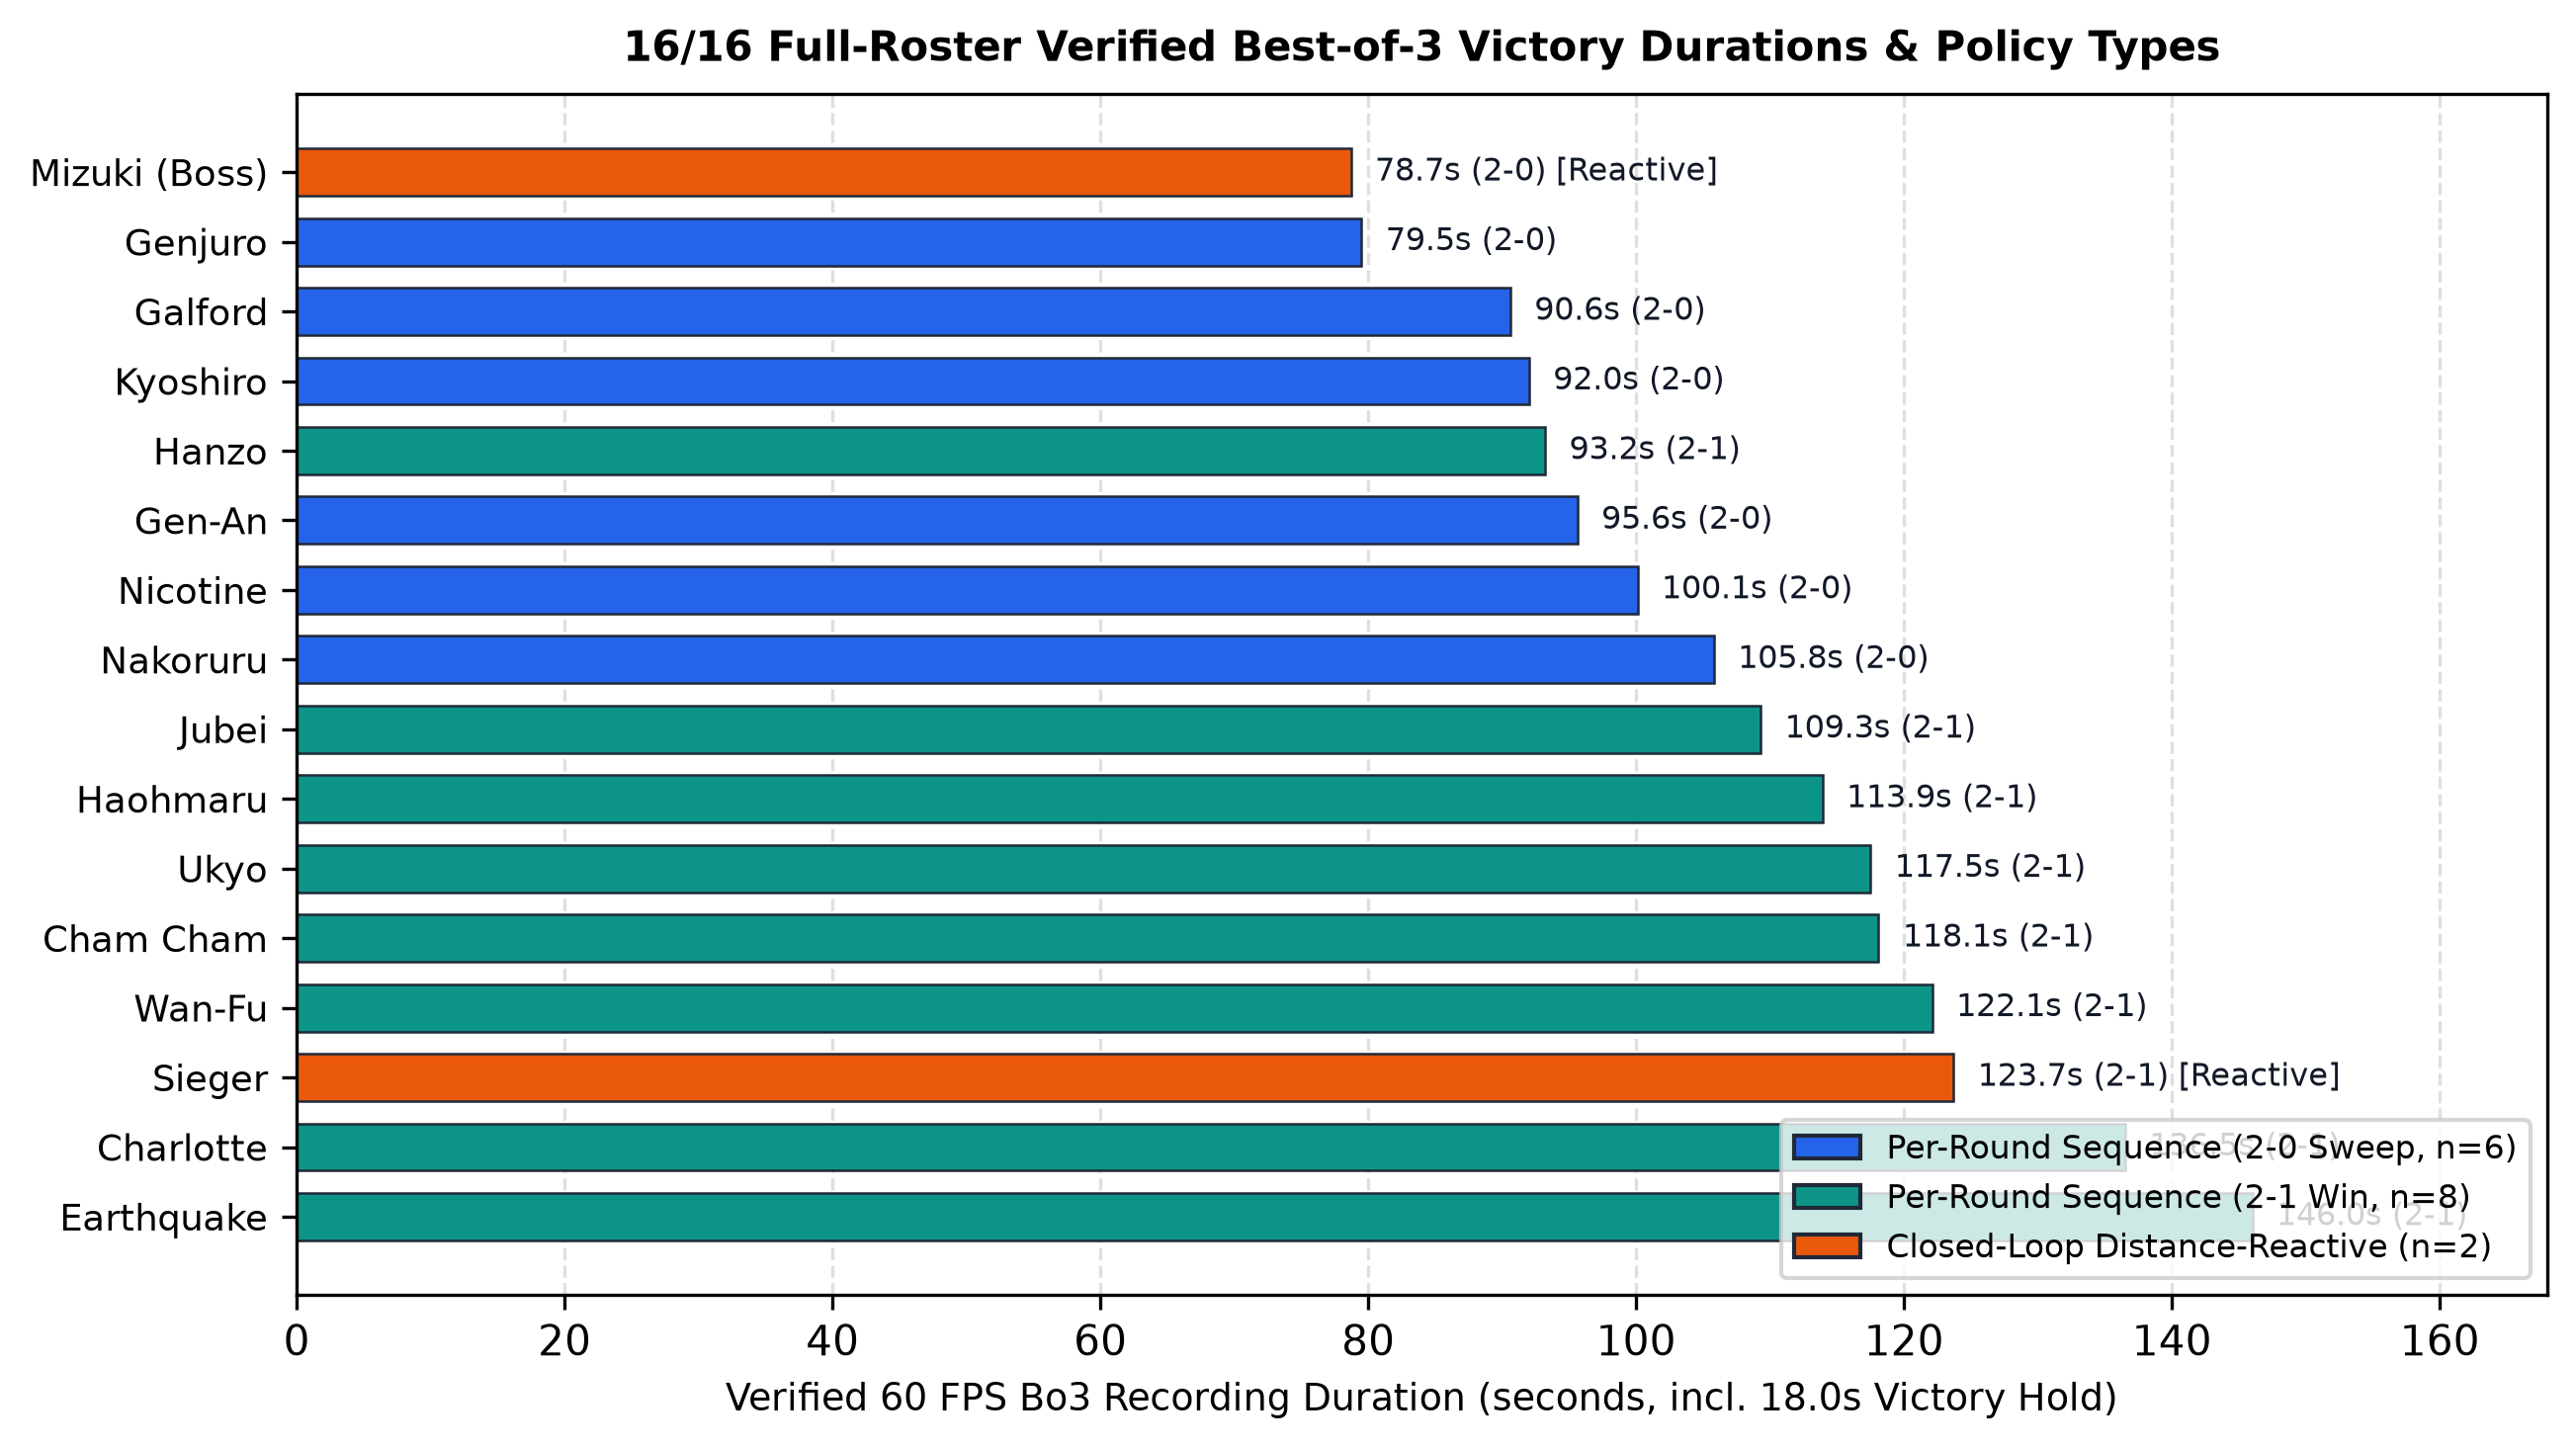
\includegraphics[width=\columnwidth]{figures/fig3_roster_performance.png}
    \caption{全员 16 位对手 60~FPS 实测 Bo3 视频时长（含 18.0~s 胜利结算停留）、最终比分及策略类型对比。}
    \label{fig:perf}
\end{figure}

\begin{table}[t]
\centering
\caption{全员 16/16 实机 Bo3 验收总表（1$\times$ 60~FPS MAME 实测）}
\label{tab:results}
\scriptsize
\begin{tabular}{r l c r r l}
\hline
\textbf{序号} & \textbf{对手角色} & \textbf{比分} & \textbf{时长(s)} & \textbf{体积(MB)} & \textbf{策略类型} \\
\hline
1  & 地震 (Earthquake)     & 2--1 & 146.0 & 30.13 & 分回合序列 \\
2  & 牙神幻十郎 (Genjuro)  & 2--0 &  79.5 & 20.15 & 分回合序列 \\
3  & 加尔福特 (Galford)    & 2--0 &  90.6 & 16.77 & 分回合序列 \\
4  & 娜可露露 (Nakoruru)   & 2--0 & 105.8 & 19.97 & 分回合序列 \\
5  & 查姆查姆 (Cham Cham)  & 2--1 & 118.1 & 21.04 & 分回合序列 \\
6  & 王虎 (Wan-Fu)         & 2--1 & 122.1 & 26.46 & 分回合序列 \\
7  & 席格 (Sieger)         & 2--1 & 123.7 & 19.50 & \textbf{距离闭环} \\
8  & 千两狂死郎 (Kyoshiro) & 2--0 &  92.0 & 17.27 & 分回合序列 \\
9  & 服部半藏 (Hanzo)      & 2--1 &  93.2 & 13.55 & 分回合序列 \\
10 & 不知火幻庵 (Gen-An)   & 2--0 &  95.6 & 19.90 & 分回合序列 \\
11 & 花讽院和仲 (Nicotine) & 2--0 & 100.1 & 15.69 & 分回合序列 \\
12 & 罗将神水姬 (Mizuki)   & 2--0 &  78.7 & 19.23 & \textbf{距离闭环} \\
13 & 霸王丸镜像 (Haohmaru) & 2--1 & 113.9 & 20.78 & 分回合序列 \\
14 & 橘右京 (Ukyo)         & 2--1 & 117.5 & 17.30 & 分回合序列 \\
15 & 柳生十兵卫 (Jubei)    & 2--1 & 109.3 & 19.14 & 分回合序列 \\
16 & 夏洛特 (Charlotte)    & 2--1 & 136.5 & 22.94 & 分回合序列 \\
\hline
\multicolumn{2}{l}{\textbf{合计 / 均值}} & \textbf{16/16} & \textbf{107.7} & \textbf{19.95} & \textbf{14 序列 / 2 闭环} \\
\hline
\end{tabular}
\end{table}

全员 16 场实机验收中，AI 霸王丸取得 7 场 2--0 零封（43.8\%）与 9 场 2--1 决胜（56.3\%），完整录像平均时长 107.7~s（范围 78.7--146.0~s）。

\subsection{真 2P VS 人机实机对抗验证}
为验证真实人机互动且彻底消除 1P/2P 抢键冲突，我们实现了真双人 VS 模式（\texttt{.\textbackslash play\_demo.ps1 -Human}）：系统自动开启街机 Freeplay（\texttt{DSW:64:1}）并注入 2P START（\texttt{role=2, mask=0x04}）触发原版“2P 乱入”选人界面；同时将 1P 键盘映射全部设为 \texttt{NONE}，将 2P 自动绑定为 \texttt{WASD + J/K/L/U/I/O}。开战瞬间由 WRAM 读取 \texttt{UID + E\_CHAR} 自动路由至对应克制专家。真人盲测既验证了 AI 霸王丸的高强度进攻压制力，也成功暴露并推动修复了硬件角色 ID 偏移（\texttt{0x0B}--\texttt{0x10}）与幻影第 2 局两处隐蔽缺陷。

\section{局限性剖析与 MoE 反哺 RL 路线}
我们坦诚指出当前系统的两项主要局限：
\begin{enumerate}
    \item \textbf{序列策略泛化边界}：14 个基于序列的专家对固定街机 CPU 状态机高度稳定，但人类玩家可通过连续下段滑铲（在真人操控查姆查姆的实测中已观察到）或极限距离骗招抓破绽。
    \item \textbf{锁步步进节奏}：当前人机模式按每 2 帧一次网桥往返步进（有效约 45--60~FPS），尚非完全异步的无阻塞推流控制。
\end{enumerate}

现有 16/16 MoE 专家库并非深度强化学习的替代品，而是其理想的冷启动底座（详见配套路线文档 \texttt{finaldoc/}）：
\begin{itemize}
    \item \textbf{行为克隆（BC）冷启动 + Critic 热身 PPO}：用 16 份 MoE 专家在 \texttt{SS2RoundEnv} 中带轻度扰动重放采集完整 50 维 \texttt{(obs, act, r, s', done)} 轨迹，经 BC 预训练导出 SB3 权重，先冻结 Actor 热身 Critic，再低学习率联训 PPO。
    \item \textbf{Kickstarting 策略蒸馏}~\cite{schmitt2018kickstarting}：在 PPO 目标中加入退火的 $\lambda(t) D_{\text{KL}}(\pi_{\text{MoE}} \,\|\, \pi_{\text{PPO}})$ 正则项，兼顾防守习惯保持与未知状态泛化。
    \item \textbf{Go-Explore 残局课程与离线 RL}~\cite{ecoffet2021goexplore,kostrikov2022iql}：从 MoE 中后盘自动沉淀残局 \texttt{.sta} 锚点实施逆向课程学习，或混合 MoE 胜局与历史 PPO 探索失败轨迹，在纯 GPU 上进行 IQL 离线训练以绕开 MAME 采样吞吐瓶颈。
\end{itemize}

\section{结论}
本文介绍了一套面向经典街机《真侍魂》的硬件感知混合专家系统架构，在单台 Windows 主机上实现了全员 16/16 实机三局两胜验证与零冲突真 2P VS 人机对抗。除 16/16 全员通关成果本身外，本文提炼的核心工程启示在于：直接 WRAM 实体感知、语义 SMDP 意图抽象、闭环距离反应控制以及物理不变量评测守卫，是构建可信格斗游戏 AI 系统的决定性支柱。完整的 92 文件纯净开源包、中英双语文档与全部验证工具已公开发布于 \url{https://github.com/footballqq/samsho2-moe-ai}。

\begin{thebibliography}{9}
\bibitem{schulman2017ppo}
J.~Schulman, F.~Wolski, P.~Dhariwal, A.~Radford, and O.~Klimov, ``Proximal policy optimization algorithms,'' \textit{arXiv preprint arXiv:1707.06347}, 2017.

\bibitem{sutton1999options}
R.~S. Sutton, D.~Precup, and S.~Singh, ``Between MDPs and semi-MDPs: A framework for temporal abstraction in reinforcement learning,'' \textit{Artificial Intelligence}, vol.~112, no.~1--2, pp.~181--211, 1999.

\bibitem{jacobs1991moe}
R.~A. Jacobs, M.~I. Jordan, S.~J. Nowlan, and G.~E. Hinton, ``Adaptive mixtures of local experts,'' \textit{Neural Computation}, vol.~3, no.~1, pp.~79--87, 1991.

\bibitem{lu2013fightingice}
F.~Lu, K.~Yamamoto, L.~H. Nomura, S.~Mizuno, Y.~Lee, and R.~Thawonmas, ``Fighting game artificial intelligence competition platform,'' in \textit{Proc. IEEE Global Conf. on Consumer Electronics (GCCE)}, 2013, pp.~320--323.

\bibitem{vinyals2019alphastar}
O.~Vinyals \textit{et al.}, ``Grandmaster level in StarCraft II using multi-agent reinforcement learning,'' \textit{Nature}, vol.~575, pp.~350--354, 2019.

\bibitem{amodei2016concrete}
D.~Amodei \textit{et al.}, ``Concrete problems in AI safety,'' \textit{arXiv preprint arXiv:1606.06565}, 2016.

\bibitem{schmitt2018kickstarting}
S.~Schmitt \textit{et al.}, ``Kickstarting deep reinforcement learning,'' \textit{arXiv preprint arXiv:1803.03835}, 2018.

\bibitem{ecoffet2021goexplore}
A.~Ecoffet, J.~Huizinga, J.~Lehman, K.~O. Stanley, and J.~Clune, ``First return, then explore,'' \textit{Nature}, vol.~590, pp.~580--586, 2021.

\bibitem{kostrikov2022iql}
I.~Kostrikov, A.~Nair, and S.~Levine, ``Offline reinforcement learning with implicit Q-learning,'' in \textit{Proc. Int. Conf. on Learning Representations (ICLR)}, 2022.
\end{thebibliography}

\end{document}
